% !TeX root = ../thesis.tex
\subsection{F\# Alea.cuBase Solution}
The F\# Alea.cuBase solution has many similarities to the CUDA C implementation.
One key factor is that the Runge-Kutta four kernel is implemented using Code Quotations (see section \ref{subsec:background:codequotations}), as are the plan-specific $dV$ and $bj\_ii$ methods.
As the plan-specific $dV$ and $bj\_ii$ typically include references to helper-methods, they could be defined in terms of Quotations and referenced using the splicing operators.
Another option is to use use the \lstinline$[<ReflectedDefinition>]$ F\# attribute on methods which make most regular methods accessible in Quotations.
An example of this can be seen in code sample \ref{cubase_pureendowment}. 
The various plans are in this case not implemented using classes (though they could have been), so each method name is prepended with a plan acronym ($pe\_$).
It also refers to some common constants and methods not defined in the class much like the previous implementations.
%\clearpage
\begin{lstlisting}[language=FSharp, caption=The pure endowment insurance plan expressed in F\# Alea.cuBase, label=cubase_pureendowment]
[<ReflectedDefinition>] 
let pe_b_0 t = zero
[<ReflectedDefinition>]
let pe_mu_01 t = GM t
[<ReflectedDefinition>]
let pe_bj_00 t = if t = pensiontime then bpension else zero
[<ReflectedDefinition>]
let pe_bj_01 t = zero
let pe_dV = 
  <@ fun t (V:deviceptr<floatP>) (res:deviceptr<floatP>) -> 
      res.[0] <- r t * V.[0] - pe_b_0 t - pe_mu_01 t * (zero - V.[0] + pe_bj_01 t) @>
let pe_bj_ii = 
  <@ fun t (res:deviceptr<floatP>) ->
      res.[0] <- pe_bj_00 t @>
\end{lstlisting}

To run the plan there is one Runge-Kutta four kernel defined as can partially be seen in code sample \ref{cubase_rk4_n_snippet}. 
For the full implementation see appendix \ref{app:cubase_rk4_n}. 
What may be of interest is the $deviceptr$ type used by $Va$ and $result$, which works very similarly to pointers in C.
The temporary arrays $k_i$, $tmp$ and $v$ may also be of interest. 
They are initiated using Alea.cuBase and then transformed into the generic $deviceptr$ type representations like $Va$ and $result$.
\clearpage
\begin{lstlisting}[language=FSharp, caption=The Runge-Kutta four solver expressed in F\# Alea.cuBase, label=cubase_rk4_n_snippet]
let RK4_n dV bj_ii states = cuda {
	let! kernel =
		<@ fun a b steps (Va:deviceptr<floatP>) (result:deviceptr<floatP>) ->
			//Calculate unique result offset
			let offset = (blockIdx.x * blockDim.x + threadIdx.x) * states * (a + 1)
            //Splice in other quotation expressions
			let dV = %dV
			let bj_ii = %bj_ii
			let h   = -one / conv steps
			//Initialize reusable intermediary arrays
			let k1	  = __local__.Array<floatP>(states) |> __array_to_ptr
			let k2	  = __local__.Array<floatP>(states) |> __array_to_ptr
			let k3	  = __local__.Array<floatP>(states) |> __array_to_ptr
			let k4	  = __local__.Array<floatP>(states) |> __array_to_ptr
			let tmp	  = __local__.Array<floatP>(states) |> __array_to_ptr
			let v	  = __local__.Array<floatP>(states) |> __array_to_ptr
            ...Actual Runge-Kutta 4 implementation
        @> |> Compiler.DefineKernel 

    return Entry(fun program ->
        let worker = program.Worker
        let kernel = program.Apply kernel
        fun a b steps blocks threads ->
            //Calculate size of result array
            let n = (a + 1) * states * blocks * threads
            //Allocate memory on device
            use Va = worker.Malloc<floatP>(Array.zeroCreate states)
            use result = worker.Malloc<floatP>(Array.zeroCreate n)
            let lp = LaunchParam (blocks, threads)
            ...Timing mechanism start
            //Launch kernel with parameters
            kernel.Launch lp a b steps Va.Ptr result.Ptr
            ...Timing mechanism end, save kernel execution time in ms
            //Gather and return device results and kernel execution time
            let result = result.Gather()
            result, ms
        )
}
\end{lstlisting}

As the GPU code is generated at runtime, a lot of the compile-time limitations of CUDA C disappear.
While the kernels may not take all types of parameters at launch-time, during kernel-compilation they can often be used.
The code is not making much use of the functional programming paradigm and memory-allocation for the device is still required.
There are however many small changes like the $use$ keyword, and not having to provide the size of the allocated memory, still make it faster and safer to program in F\# as opposed to CUDA C.

The solution also makes use of a method to compile the kernels for reuse and another to execute them, as can be seen in code sample \ref{cubase_compileandrun}. 

\begin{lstlisting}[language=FSharp, caption=Kernel compilation and execution methods in F\# Alea.cuBase, label=cubase_compileandrun]
let compile dV bj_ii states = RK4_n dV bj_ii states |> Compiler.load Worker.Default

let runKernel (program:Program<int->int->int->int->int->floatP[]*float>) a b blocks threads = program.Run a b steps blocks threads
\end{lstlisting}

The results of running the F\# Alea.cuBase solution shows that the highest number of calculations per ms were \emph{98.33} for single precision and \emph{25.30} per ms for double precision.
For the full single-precision results table \ref{table:cubaseManualfloattime} and for double precision results see table \ref{table:cubaseManualdoubletime}.
For the entire results, see appendix \ref{app:cuBase_manual_runtimes}.
This is a slight improvement over the CUDA C single precision version while being nearly identical for double precision.
%Unlike the CUDA C version, I was not able to limit the maximum amount of registers used, making it impossible to test configurations with more than 512 threads.
The documented way to limit the maximum number of registers in Alea.cuBase did not work, so it was impossible to run double precision configurations with 1024 threads.

For more information on result comparison see section \ref{subsec:result_comparison}.

\begin{table}[h!]
\centering
{\setlength{\extrarowheight}{2pt}{\setlength{\tabcolsep}{3pt}
\begin{tabular}{ | r | r | r | r | r | r | r | r | }
  \hline
\diaghead{Threads/Blocks}{Threads}{Blocks}
		&	1		& 	14 	 	&	14*5 	& 	14*10 	& 	14*20 	& 	14*25 	& 	14*30 	\\ \hline
1		& 	0.02	&	0.34 	&	1.61	&	1.67	&	2.15	&	2.04	&	2.36	\\ \hline
8		& 	0.19	&	2.72 	&	12.87	&	13.33	&	17.13	&	16.28	&	18.80	\\ \hline
16		&	0.38	&	5.43	&	25.60	&	26.53	&	34.05	&	32.35	&	37.47	\\ \hline
32		&	0.76	&	10.78	&	50.58	&	52.59	&	67.61	&	64.27	&	74.51	\\ \hline
64		&	1.37	&	21.12	&	67.15	&	70.75	&	88.71	&	85.95	&	95.53	\\ \hline
128		&	1.69	&	37.36	&	77.74	&	84.81	&	85.36	&	88.89	&	92.55	\\ \hline
256		&	1.73	&	46.54	&	95.53	&	97.41	&	97.92	&	94.80	&	95.49	\\ \hline
512		&	6.75	&	48.20	&	97.44	&	98.01	&	98.23	&	96.28	&	98.31	\\ \hline
1024	&	6.93	&	96.11	&	97.94	&	98.16	&	98.31	&	98.33	&	98.29	\\ \hline
\end{tabular}}}
\caption{F\# Alea.cuBase calculations per ms with single precision\label{table:cubaseManualfloattime}}
\end{table}

\begin{table}[h!]
\centering
{\setlength{\extrarowheight}{2pt}{\setlength{\tabcolsep}{3pt}
\begin{tabular}{ | r | r | r | r | r | r | r | r | }
  \hline
\diaghead{Threads/Blocks}{Threads}{Blocks}
		&	1		&	14		&	14*5	&	14*10	&	14*20	&	14*25	&	14*30	\\ \hline
1		&	0.01	&	0.11	&	0.49	&	0.49	&	0.63	&	0.59	&	0.69	\\ \hline
8		&	0.06	&	0.87	&	3.93	&	3.91	&	5.01	&	4.74	&	5.51	\\ \hline
16		&	0.12	&	1.73	&	7.83	&	7.88	&	10.05	&	9.48	&	11.01	\\ \hline
32		&	0.25	&	3.46	&	15.63	&	15.75	&	20.06	&	18.94	&	22.02	\\ \hline
64		&	0.49	&	6.73	&	19.96	&	21.67	&	24.42	&	23.22	&	25.22	\\ \hline
128		&	0.96	&	11.26	&	20.31	&	25.18	&	24.10	&	24.94	&	25.34	\\ \hline
256		&	1.61	&	12.53	&	24.84	&	25.12	&	25.27	&	25.35	&	25.42	\\ \hline
512		&	1.79	&	25.03	&	25.26	&	25.28	&	25.30	&	25.30	&	25.25	\\ \hline
\end{tabular}}}
\caption{F\# Alea.cuBase calculations per ms with double precision\label{table:cubaseManualdoubletime}}
\end{table}

\subsection{Insurance plan parameterization}\label{sub:manual_parameterization}
The parallelized versions have so far been running the same static plans over and over again which is not very useful in practical scenarios.
To make parallellisation useful, the ability to make constants parameterized is required.
These constants could for example be the interest rate or the age of the insured.

To add this parameterization, the $dV$ and $bj\_ii$ method signatures were changed to include an additional array containing parameters for the insurance plan.
The life insurance plan implementations were then made responsible for knowing how many variables there were and which variables mapped to which position in the parameter array. 
They also had to pass the parameters to the methods that required them, for example the age to the mortality functions.
This iteration of the code also switched to using classes eliminating the need for prepending prefixes to the various plan methods.
For an example of this, see code sample \ref{cubase_pureendowmentparams}.
The RK4\_n kernel was also altered to provide the thread-specific pointer to the plan parameter array and pass this to the updated $dV$ and $bj\_ii$ methods.
This position would be the position of the thread multiplied by the number of plan parameters.
For a brief overview of the changes to the RK4\_n kernel, see code sample \ref{cubase_rk4nparams}.

\begin{lstlisting}[language=FSharp, caption=Parameterized pure endowment life insurance plan in F\# Alea.cuBase, label=cubase_pureendowmentparams]
type PureEndowment (planParams, paramCount) =
  inherit Plan<floatP>(40, 0, 1, planParams, paramCount) with
    [<ReflectedDefinition>]
    let b_0 t = conv 0
    
    [<ReflectedDefinition>]
    let mu_01 t age = GM t age
    
    [<ReflectedDefinition>]
    let bj_00 t pensiontime bpension = if t = pensiontime then bpension else conv 0

    [<ReflectedDefinition>]
    let bj_01 t = conv 0

    override this.dV = <@ fun t (V:deviceptr<floatP>) (planParams:deviceptr<floatP>) (res:deviceptr<floatP>) -> 
      let age = planParams.[0]
      res.[0] <- (r t) * V.[0] - (b_0 t) - (mu_01 t age) * (conv 0 - V.[0] + (bj_01 t))
      @>
    override this.bj_ii = <@ fun t (planParams:deviceptr<floatP>) (res:deviceptr<floatP>) -> 
      let bpension = planParams.[1]                
      let pensiontime = planParams.[2]
      res.[0] <- bj_00 t pensiontime bpension
      @>
\end{lstlisting}

\begin{lstlisting}[language=FSharp, caption=Parameterized RK4\_n kernel changes in F\# Alea.cuBase, label=cubase_rk4nparams]
let RK4_n (plan:Plan<_>) = cuda {
  let! kernel =
    <@ fun (a:int) b steps (Va:deviceptr<floatP>) (d_params:deviceptr<floatP>) (result:deviceptr<floatP>) ->
      if blockIdx.x * blockDim.x + threadIdx.x > plan.planParams.Length/plan.paramCount then () else

      let localParams = d_params.Ptr ((threadIdx.x + blockIdx.x*blockDim.x)*plan.paramCount)
      while y > b do
        bj_ii (conv y) localParams v
        for s = 0 to steps - 1 do
          dV (if s = 0 then t - limit else t) v localParams k1
          dV (t + h / conv 2) tmp localParams k2
          dV (t + h / conv 2) tmp localParams k3
          dV (if s = steps - 1 then t + h + limit else t + h) tmp localParams k4
        y <- y - 1
    @> |> Compiler.DefineKernel 

  return Entry(fun program ->
    fun a b steps blocks threadsPerBlock ->
      use planParams = worker.Malloc<'T>(plan.planParams)
      let msec, _ = time false "" (fun () -> kernel.Launch lp a b steps Va.Ptr planParams.Ptr result.Ptr)
    )
}
\end{lstlisting}
%\clearpage
The parameters were shaped so each thread would have its own unique set of parameters laid in sequence. 
See figure \ref{fig:ParameterizationVisualization} for a visualized example of this.

\begin{figure}[h!]\centering
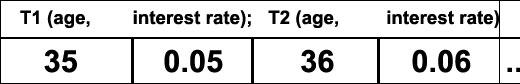
\includegraphics[scale=0.4]{ParameterizationVisualization.jpg}
\caption{Parameterization visualization for the variables age and interest rate for threads T1 and T2.\label{fig:ParameterizationVisualization}}
\end{figure}

Results were slightly slower for floats with the highest number of calculations per second being \emph{95.26} calculations per ms, but almost twice as fast for doubles with \emph{54.53} calculations per ms. 
For the remaining iterations per ms results see tables \ref{table:cubaseManualParamsfloattime} and \ref{table:cubaseManualParamsdoubletime} for single and double precision respectively.
For the runtimes see appendix \ref{app:cuBase_manual_params_runtimes}.
The performance increase in the double results are likely because less of the functions rely on constants defined outside the functions themselves, instead relying on passing the parameters to the function. %this explanation is still shit
This is likely something that can be used for further projects. %test this

The results of the test shows that parameters not only barely affect the running time and are therefore more than viable, it also shows that the double results in particular can be optimized a good bit which increases their viability significantly.

\begin{table}[h!]
\centering
{\setlength{\extrarowheight}{2pt}{\setlength{\tabcolsep}{3pt}
\begin{tabular}{ | r | r | r | r | r | r | r | r | } \hline
\diaghead{Threads/Blocks}{Threads}{Blocks}
	&	1		&	14		&	14*5	&	14*10	&	14*20	&	14*25	&	14*30	\\ \hline
1	&	0.02	&	0.32	&	1.53	&	1.60	&	2.09	&	1.99	&	2.33	\\ \hline
8	&	0.19	&	2.59	&	12.17	&	12.70	&	16.56	&	15.80	&	18.30	\\ \hline
16	&	0.37	&	5.13	&	24.07	&	25.09	&	32.71	&	31.29	&	36.43	\\ \hline
32	&	0.71	&	10.00	&	46.89	&	48.79	&	63.86	&	60.94	&	70.47	\\ \hline
64	&	1.43	&	19.66	&	62.13	&	69.81	&	85.64	&	82.79	&	90.86	\\ \hline
128	&	2.82	&	34.63	&	70.70	&	68.48	&	90.20	&	86.77	&	92.09	\\ \hline
256	&	5.09	&	43.36	&	82.92	&	87.60	&	94.94	&	94.27	&	94.98	\\ \hline
512	&	6.37	&	45.93	&	94.01	&	93.44	&	95.28	&	94.93	&	95.38	\\ \hline
1024&	6.64	&	92.45	&	94.76	&	95.06	&	95.22	&	95.26	&	95.24	\\ \hline
\end{tabular}}}
\caption{F\# Alea.cuBase calculations per ms with single precision and parameters\label{table:cubaseManualParamsfloattime}}
\end{table}

\begin{table}[h!]
\centering
{\setlength{\extrarowheight}{2pt}{\setlength{\tabcolsep}{3pt}
\begin{tabular}{ | r | r | r | r | r | r | r | r | }
  \hline
\diaghead{Threads/Blocks}{Threads}{Blocks}
	&	1		&	14		&	14*5	&	14*10	&	14*20	&	14*25	&	14*30	\\ \hline
1	&	0.01	&	0.11	&	0.49	&	0.49	&	0.63	&	0.59	&	0.69	\\ \hline
8	&	0.06	&	0.85	&	3.88	&	3.92	&	5.03	&	4.72	&	5.49	\\ \hline
16	&	0.12	&	1.71	&	7.75	&	7.83	&	10.05	&	9.60	&	11.13	\\ \hline
32	&	0.24	&	3.41	&	15.46	&	15.64	&	20.87	&	25.19	&	27.01	\\ \hline
64	&	0.49	&	6.67	&	19.76	&	22.31	&	35.96	&	37.82	&	41.45	\\ \hline
128	&	0.95	&	11.16	&	22.17	&	35.49	&	44.02	&	46.82	&	48.74	\\ \hline
256	&	1.60	&	12.01	&	33.78	&	43.26	&	49.77	&	51.62	&	52.69	\\ \hline
512	&	1.78	&	24.74	&	40.93	&	48.12	&	52.79	&	53.82	&	54.53	\\ \hline
\end{tabular}}}
\caption{F\# Alea.cuBase calculations per ms with double precision and parameters\label{table:cubaseManualParamsdoubletime}}
\end{table}

%todo:?
%RK4 step image
%delta numerical critique
%visual ast of quotation?